\documentclass[a4paper,11pt]{report}
\usepackage[latin1]{inputenc}
\usepackage[T1]{fontenc}
\usepackage[english]{babel}
\usepackage{float}
\usepackage{hyperref}
\usepackage{listings}
\usepackage{cite}
\usepackage{acro}
\usepackage{graphicx}
\usepackage[nodayofweek]{datetime}

\acsetup{first-style=short}
\DeclareAcronym{rl}{
  short = RL ,
  long  = Reinforcement Learning,
  class = abbrev
}
\DeclareAcronym{ai}{
  short = AI ,
  long  = Artificial Intelligence,
  class = abbrev
}


\DeclareGraphicsRule{*}{mps}{*}{}

% Commands
\newcommand{\HRule}{\rule{\linewidth}{0.5mm}} % Defines a new command for the horizontal lines

\begin{document}

	\begin{titlepage}
		\begin{centering}
		 
		%	HEADING SECTIONS
		
		\textsc{\textbf{\LARGE{Decision making using deep reinforcement learning}}}\\[0.5cm]

		\textbf{\textit{\large{A Project Report}}}\\[1.5cm]

		\large{submitted in partial fulfilment for the award of the degree of Bachelor of Technology in Computer Science and Engineering}\\[1.5cm]

		\large{by}\\[0.5cm]

		\textbf{Jayadeep K M     (13400030)}\\
		\textbf{Kevin Joseph     (13400032)}\\
		\textbf{Mohammed Nisham K     (13400038)}\\[1.5cm]
		
		{under the guidance of}\\[0.25cm]
		\large{Mr. Vipin Vasu A V}\\[0.5cm]

		
\includegraphics[width=5cm]{images/logo.jpg} 

		\textsc{Department of Computer Science and Engineering}\\
		\textsc{College of Engineering Trivandrum}\\
		\textsc{Kerala}\\[0.5cm]
		\textsc{May 2017}\\
		\vfill % Fill the rest of the page with whitespace
		\end{centering}
	\end{titlepage}

	\begin{titlepage}
		\begin{centering}
			\textsc{\large{Department of Computer Science and Engineering}}\\
			\textsc{\large{College of Engineering Trivandrum}}\\[0.5cm]

			
\includegraphics[width=5cm]{images/logo.jpg}\\[0.5cm]
			\textbf{\textit{\LARGE\textsc{{certificate}}}}\\[0.3cm]

		\end{centering}

		\begin{sloppypar}
		\large{This is to certify that the report entitled ``Decision making using deep reinforcement learning'' is a bonafide record of the project work done by \textbf{Jayadeep K M} (13400030), \textbf{Kevin Joseph} (13400032) and \textbf{Mohammed Nisham K} (13400038) under my supervision and guidance, in partial fulfilment for the award of the degree of Bachelor of Technology in Computer Science and Engineering from the University of Kerala in the year 2017.}\\[1.5cm]
		\end{sloppypar}

		\begin{minipage}{0.5\textwidth}
		\begin{flushleft}
		\begin{centering} \large
			\large{Mrs. Liji}\\
			\small{\textit{\textbf{Professor and Head}}}\\
			\small{\textit{\textbf{Dept. of Computer Science and Engineering}}}\\
		\end{centering}
		\end{flushleft}
		\end{minipage}
		~
		\begin{minipage}{0.5\textwidth}
		\begin{centering} \large
		\large{Mr. Vipin Vasu A V}\\
		\small{(Guide)}\\
		\small{\textit{\textbf{Asst. Professor}}}\\
		\small{\textit{\textbf{Dept. of Computer Science and Engineering}}}\\[1.5cm]

		\end{centering}
		\end{minipage}\\[1.0cm]

		\begin{flushleft}
		Place: Trivandrum\\
		Date:  11-05-2017\\
		\end{flushleft}
		\vfill % Fill the rest of the page with whitespace
	\end{titlepage}

	% TODO Ack before this
	\pagenumbering{roman}
	
	\begin{abstract}
		Creating a general purpose AI has been an area of research since the beginning of computers and programming. Reinforcement learning is a major step towards a general purpose AI. \\

		This project is aimed at creating a program that can learn to make decisions in an environment that is defined by a high-dimensional input, and has sparce and time delayed rewards for these actions. Such programs can be useful in problems where decsion must be made based on high dimensional sensory input such as camera feed. This project uses Q-learning algorithm to assign a quality value to each action in a state of the environment. \\

		Atari games are used to demonstrate this approach, by training the program to play breakout game for upto 50 epochs and observing performance improvement. The trained neural network was saved and tested at the end of every epoch. The performance parameters like average q-value, average reward, games per epoch were also saved. The performace parameters showed a clear rise in performace for breakout (50 epochs) and space invaders (8 epochs). \\

		The project has applications in the field of IOT, security, gaming, stock market analysis and traffic control systems. Any system that can be modelled as an environment with actions and rewards can be trained using this algorithm.

	\end{abstract}
	
	\newpage
	\tableofcontents
	\newpage
	\listoffigures
	\newpage
	\printacronyms[include-classes=abbrev,name=Abbreviations]

	\pagenumbering{arabic}
	\chapter{Introduction}
		\section{Motivation and Overview}
			Learning to control agents directly from high-dimensional sensory inputs like vision and speech is one of the long-standing challenges of Artificial Intelligence and Machine Learning. Most successful \ac{ai} applications have relied on hand-crafted features combined with linear value functions or policy representations. Clearly, the performance of such systems heavily relies on the quality of the feature representation.

			Recent advances in deep learning have made it possible to extract high-level features from raw sensory data, leading to breakthroughs in computer vision and speech recognition. These methods utilise a range of neural network architectures, including convolutional networks, multilayer perceptrons, restricted Boltzmann machines and recurrent neural networks, and have exploited both supervised and unsupervised learning.
	
			However the main advantage of Reinforcement Learning is that it does't need huge amounts of hand-labelled data and does not depend too much on the feature representation. It learns from a reward signal that maybe delayed, noisy and sparse. The delay between actions and the rewards, which maybe thousands of timesteps seems like a particularly hard problem in \ac{rl} when compared to direct association between action and reward in supervised learning. Another issue is that most problems consider all the data samples independent of each other, but in this case we need to consider the fact that the reward at the end of a session is not just the result of the last action but the result of the sequence of actions from the start of the session.

			This project is aimed at using a Convolution Neural Network along with the Q-learning algorithm to solve the above problems and make decisions based on video input from the Atari Learning Environment. Our goal is to create a single neural network agent that is able to successfully learn to play atleast 2 games with no change in agent algorithm. The network was not provided with any game-specific information or hand-designed visual features, and was not privy to then internal state of the emulator, it learned from nothing but the video input, the reward and terminal signals, and the set of possible actions just as a human player would.

			In the second chapter we discuss about the background of Deep Mind and Reinforced learning. We also discuss about the importance and advantages of decision making algorithm using reinforced learning. In the third chapter, the materials and methodologies used for the project is discussed. It includes the Algorithms used in the project, Structure of neural networks, Interface used for demonstration and code review of the project. In the fourth chapter the results of the algorithm are analyzed by plotting graphs of Atari Breakout and Space Invaders. The fifth chapter discuss about how we can extend this work and implement the algorithm on a real world scenario by taking an example of Traffic Light Control. The fifth and final chapter concludes the project.


	\chapter{Background and Literature Survey}
		\section{Deep Mind and Reinforcement Learning}

			The presented method and algorithm was first presented in a paper by a company Deep Mind which was later aquired by Google. The paper presented the algorithm as a general purpose RL algorithm that could play seven of the atari 2600 games, it showed human level play in four and super human play in three of them.
			Consider the game Breakout. In this game you control a paddle at the bottom of the screen and have to bounce the ball back to clear all the bricks in the upper half of the screen. Each time you hit a brick, it disappears and your score increases you get a reward.

			\begin{figure}[!ht]
				\begin{centering}
					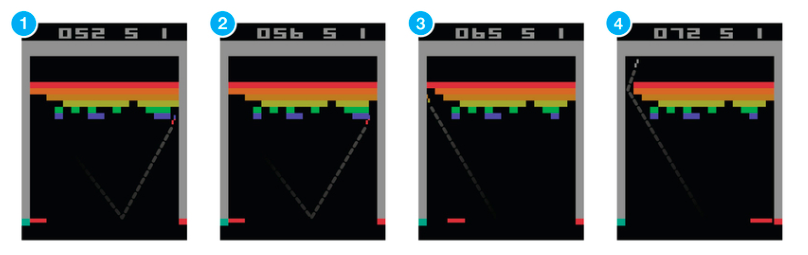
\includegraphics[width=10cm]{../Design/images/breakout.png}\\
					\caption{Breakout screens.}
				\end{centering}
			\end{figure}
			Suppose you want to teach a neural network to play this game. Input to your network would be screen images, and output would be one of four actions left, right, do nothing or fire to launch the ball. It would make sense to treat it as a classification problem for each game screen you have to decide, Which action to take. Sounds straightforward, Sure, but then you need training examples, and a lots of them. Of course you could go and record game sessions using expert players, but thats not really how we learn. We dont need somebody to tell us a million times which move to choose at each screen. We just need occasional feedback that we did the right thing and can then figure out everything else ourselves.

			This is the task reinforcement learning tries to solve. Reinforcement learning lies somewhere in between supervised and unsupervised learning. Whereas in supervised learning one has a target label for each training example and in unsupervised learning one has no labels at all, in reinforcement learning one has sparse and time-delayed labels, the rewards. Based only on those rewards the agent has to learn to behave in the environment.

			While the idea is quite intuitive, in practice there are numerous challenges. For example when you hit a brick and score a reward in the Breakout game, it often has nothing to do with the actions (paddle movements) you did just before getting the reward. All the hard work was already done, when you positioned the paddle correctly and bounced the ball back. This is called the credit assignment problem i.e., which of the preceding actions was responsible for getting the reward and to what extent.

			Once you have figured out a strategy to collect a certain number of rewards, should you stick with it or experiment with something that could result in even bigger rewards? In the above Breakout game a simple strategy is to move to the left edge and wait there. When launched, the ball tends to fly left more often than right and you will easily score about 10 points before you die. Will you be satisfied with this or do you want more? This is called the explore-exploit dilemma should you exploit the known working strategy or explore other, possibly better strategies.

			Reinforcement learning is an important model of how we (and all animals in general) learn. Praise from our parents, grades in school, salary at work these are all examples of rewards. Credit assignment problems and exploration exploitation dilemmas come up every day both in business and in relationships. Thats why it is important to study this problem, and games form a wonderful sandbox for trying out new approaches.

	\chapter{Materials and Methodology}
		\section{Algorithms}
			\subsection{Markov Decision Process}
				Suppose you are an agent, situated in an environment (e.g. Breakout game). The environment is in a certain state (e.g. location of the paddle, location and direction of the ball, existence of every brick and so on). The agent can perform certain actions in the environment (e.g. move the paddle to the left or to the right). These actions sometimes result in a reward (e.g. increase in score). Actions transform the environment and lead to a new state, where the agent can perform another action, and so on. The rules for how you choose those actions are called policy. The environment in general is stochastic, which means the next state may be somewhat random (e.g. when you lose a ball and launch a new one, it goes towards a random direction).
				\begin{figure}[!ht]
					\begin{centering}
						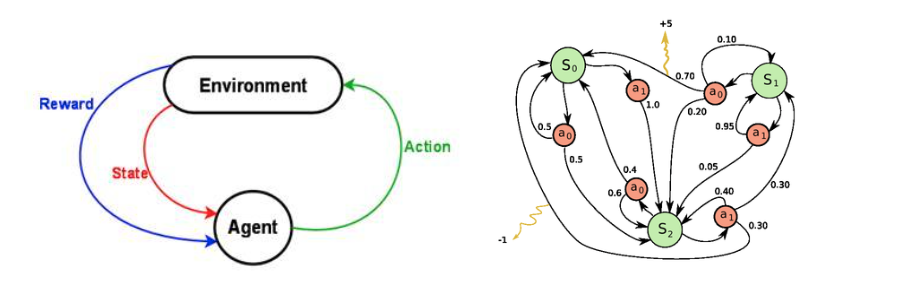
\includegraphics[width=10cm]{../Design/images/mdp.png}\\
						\caption{Markov Decision Process.}
					\end{centering}
				\end{figure}

				The set of states and actions, together with rules for transitioning from one state to another, make up a Markov decision process. One episode of this process (e.g. one game) forms a finite sequence of states, actions and rewards:

				\[ s_0,a_0,r_1,s_1,a_1,r_2,s_2, ... ,s_{n-1},a_{n-1},r_n,s_n\]

				Here s$_{i}$ represents the state, a$_i$ is the action and r$_{i+1}$ is the reward after performing the action. The episode ends with terminal state sn (e.g. game over screen). A Markov decision process relies on the Markov assumption, that the probability of the next state si+1 depends only on current state si and action ai, but not on preceding states or actions.
			\subsection{Discounted Future Reward}
				To perform well in the long-term, we need to take into account not only the immediate rewards, but also the future rewards we are going to get. How should we go about that?

				Given one run of the Markov decision process, we can easily calculate the total reward for one episode:

				\[ R = r_1 + r_2 + r_3 + ... + r_n \]

				Given that, the total future reward from time point t onward can be expressed as:

				\[ R_t = r_t + r_{t+1} + r_{t+2} + ... + r_n \]

				But because our environment is stochastic, we can never be sure, if we will get the same rewards the next time we perform the same actions. The more into the future we go, the more it may diverge. For that reason it is common to use discounted future reward instead:

				\[ R_t = r_t + {\gamma}r_{t+1} + {\gamma}^2r_{t+2} + ... + {\gamma}^{n-t}r_n\]

				Here Y is the discount factor between 0 and 1 the more into the future the reward is, the less we take it into consideration. It is easy to see, that discounted future reward at time step t can be expressed in terms of the same thing at time step t+1:

				\[ R_t = r_t + \gamma(r_{t+1} + \gamma(r_{t+2} + ...)) = r_t + {\gamma}R_{t+1}\]

				If we set the discount factor Y=0, then our strategy will be short sighted and we rely only on the immediate rewards. If we want to balance between immediate and future rewards, we should set discount factor to something like Y=0.9. If our environment is deterministic and the same actions always result in same rewards, then we can set discount factor $\gamma$=1.

				A good strategy for an agent would be to always choose an action that maximizes the (discounted) future reward.
			\subsection{Q-Learning}
				In Q-learning we define a function Q(s, a) representing the maximum discounted future reward when we perform action a in state s, and continue optimally from that point on.

				\[ Q(s_t, a_t) = max R_{t+1}\]

				The way to think about Q(s, a) is that it is the best possible score at the end of the game after performing action a in state s. It is called Qfunction, because it represents the quality of a certain action in a given state.

				This may sound like quite a puzzling definition. How can we estimate the score at the end of game, if we know just the current state and action, and not the actions and rewards coming after that? We really cant. But as a theoretical construct we can assume existence of such a function. Just close your eyes and repeat to yourself five times: Q(s, a) exists, Q(s, a) exists, . Feel it?

				If youre still not convinced, then consider what the implications of having such a function would be. Suppose you are in state and pondering whether you should take action a or b. You want to select the action that results in the highest score at the end of game. Once you have the magical Q-function, the answer becomes really simple pick the action with the highest Q value!

				\[ \pi(s) = argmax_a Q(s,a) \]

				The above policy, the rule how we choose an action in each state.
				OK, how do we get that Q function then? Lets focus on just one transition <s, a, r, s>. Just like with discounted future rewards in the previous section, we can express the Q value of state s and action a in terms of the Q value of the next state s.

				\[ Q(s,a) = r + {\gamma}max_{a'}Q(s',a')\]

				This is called the Bellman equation. If you think about it, it is quite logical maximum future reward for this state and action is the immediate reward plus maximum future reward for the next state.
				The main idea in Q-learning is that we can iteratively approximate the Q-function using the Bellman equation. In the simplest case the Q-function is implemented as a table, with states as rows and actions as columns. The gist of the Q learning algorithm is as simple as the following:

				\begin{lstlisting}[mathescape=true, morekeywords={repeat, until}]
initialise Q[num_states, num_actions] arbitrarily
observe initial state s
repeat
	select and carry out an action a
	observe reward r and new state s'
	Q[s,a] = Q[s,a] + $\alpha$(r+ $\gamma$max$_{a'}$Q[s', a'] - Q[s,a])
	s= s'
until terminated
				\end{lstlisting}

			\subsection{Q Learning to Deep Q Network}
				Although a simple game with small number of states like tic tac toe can be easily implemented using a Q table data structure, the same approach does not work for an Atari game.

				The state of the environment in the Breakout game can be defined by the location of the paddle, location and direction of the ball and the presence or absence of each individual brick. But for something more universal, the obvious choice is screen pixels. They implicitly contain all of the relevant information about the game situation, except for the speed and direction of the ball. Two consecutive screens would have these covered as well.\\

				Taking our input of 84x84x4 pixels, In greyscale each pixel can have 128 values (atari could only emulate 128 colours), This would mean that the number of states is 128$^{84x84x4}$ which is more than the no of stars in the universe. Hence representing it in a Q table is out of the question.

				Since there are a lot of states, repetitions of states are very rare, Q table does poorly on states that it has never encountered before, While a neural network will give us an approximate value for an unknown state based on its current learning. 

				The time complexity of both Q table and Neural network remain the same at O(1) after completion of training, Although neural network might be a bit slower on account of the forward propagation it has to complete.


				Thus a shift from Q table approach to Deep Q network is done for the reasons
				\begin{itemize}
				\item Space complexity is containable even when number of states is very large
				\item Better approximation in un-encountered states
				\item Faster training with lesser data
				\end{itemize}
			\subsection{Deep Q-Learning}
				\subsubsection{Convolution Neural Networks}
					Neural networks are exceptionally good at coming up with good features for highly structured data. We could represent our Q function with a neural network, that takes the state (four game screens) and action as input and outputs the corresponding Q value. Alternatively we could take only game screens as input and output the Q-value for each possible action. This approach has the advantage, that if we want to perform a Q value update or pick the action with the highest Q value, we only have to do one forward pass through the network and have all Q values for all actions available immediately.

					Considering the fact that our input is an image input, we use a convolutional neural network. A convolutional network neuron functions similar to an optic neuron in the human brain. Each neuron instead of looking over the whole image, looks over only a small neighbourhood, and the combined effect of all the neurons performs the expected function.

					\begin{figure}[!ht]
						\begin{centering}
							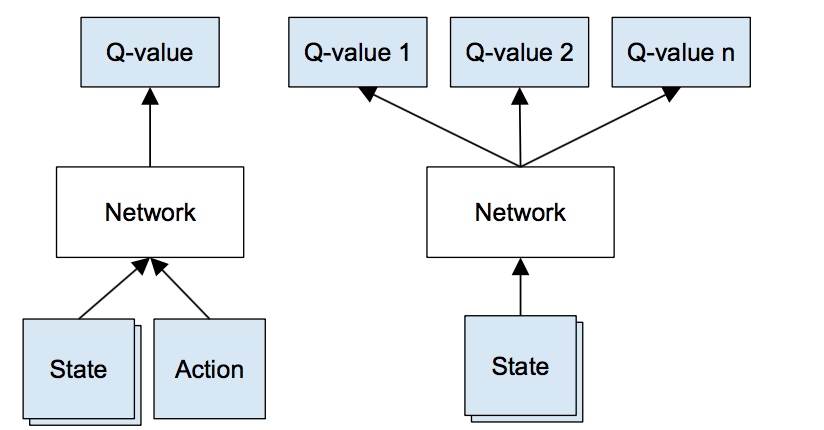
\includegraphics[width=10cm]{../Design/images/deep.png}\\
							\caption{Two Possible models for Network.}
						\end{centering}
					\end{figure}

					\begin{figure}[!ht]
						\begin{centering}
							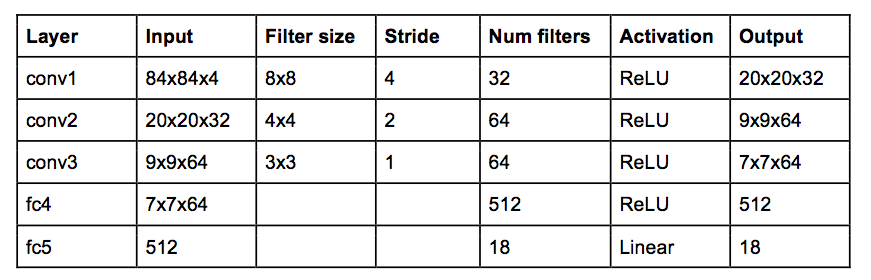
\includegraphics[width=10cm]{../Design/images/deep2.png}\\
							\caption{Network Design.}
						\end{centering}
					\end{figure}

					\begin{figure}[!ht]
						\begin{centering}
							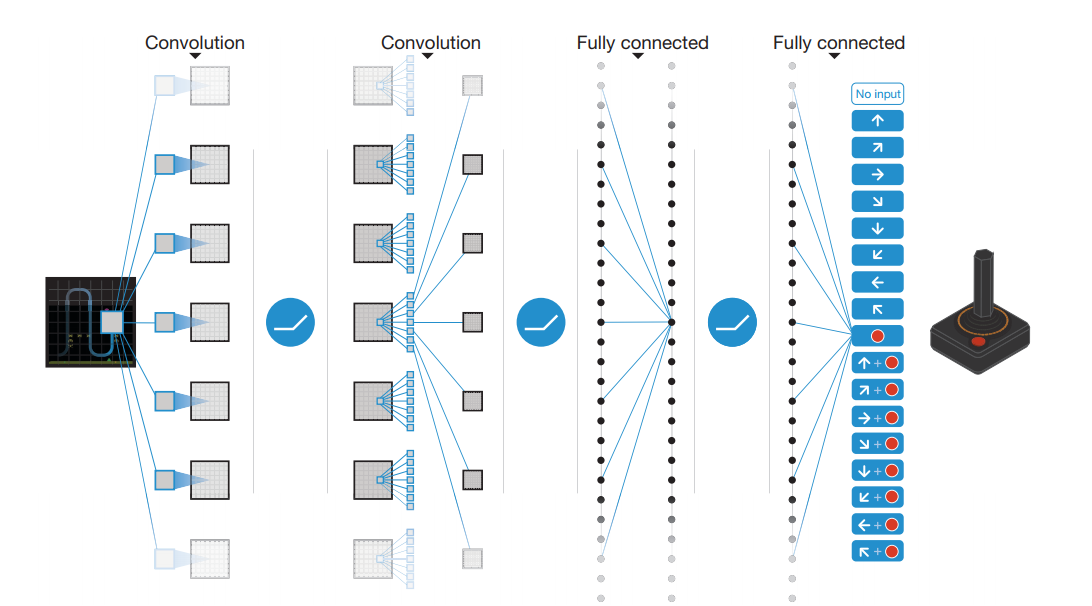
\includegraphics[width=10cm]{../Design/images/deep4.png}\\
							\caption{Layer Representation}
						\end{centering}
					\end{figure}
		\section{Atari 2600}
		The Atari 2600 (or Atari VCS before 1982) is a home video game console released on September 11, 1977, by Atari, Inc. It is credited with popularizing the use of microprocessor-based hardware and ROM cartridges containing game code, a format first used with the Fairchild Channel F video game console in 1976. This format contrasts with the older model of having non-microprocessor dedicated hardware, which could only play the games that were physically built into the unit.

		The console was originally sold as the Atari VCS, an abbreviation for Video Computer System. Following the release of the Atari 5200 in 1982, the VCS was renamed to the ``Atari 2600'', after the unit's Atari part number, CX2600. The 2600 was typically bundled with two joystick controllers, a conjoined pair of paddle controllers, and a game cartridge: initially Combat, and later Pac-Man.
		\subsection{Controls}
		The Atari 2600 comes with a joystick controller consisting of a d-pad joystick and a fire button. The joystick can move in 8 different direction and the fire button can be pressed with or without joystick movement, those along with no-move present the 18 valid controls available in Atari.

		\subsection{Screen}
		Atari emulator consists of a 160x192 pixel screen, (though mostly it is converted into a square for use), The small input size can be further reduced by converting the screen to greyscale and decreasing image resolution to 84x84 pixels, Transient data is included by including multiple screens (4). 

		Thus the atari games are perfect for deep learning due to their small input size (84x84x4) and small output size (18) which works well with a deep neural network.
		
		\newpage
		\section{Program Development}
			\subsection{Class Diagram}
				\begin{figure}[H]
					\begin{centering}
						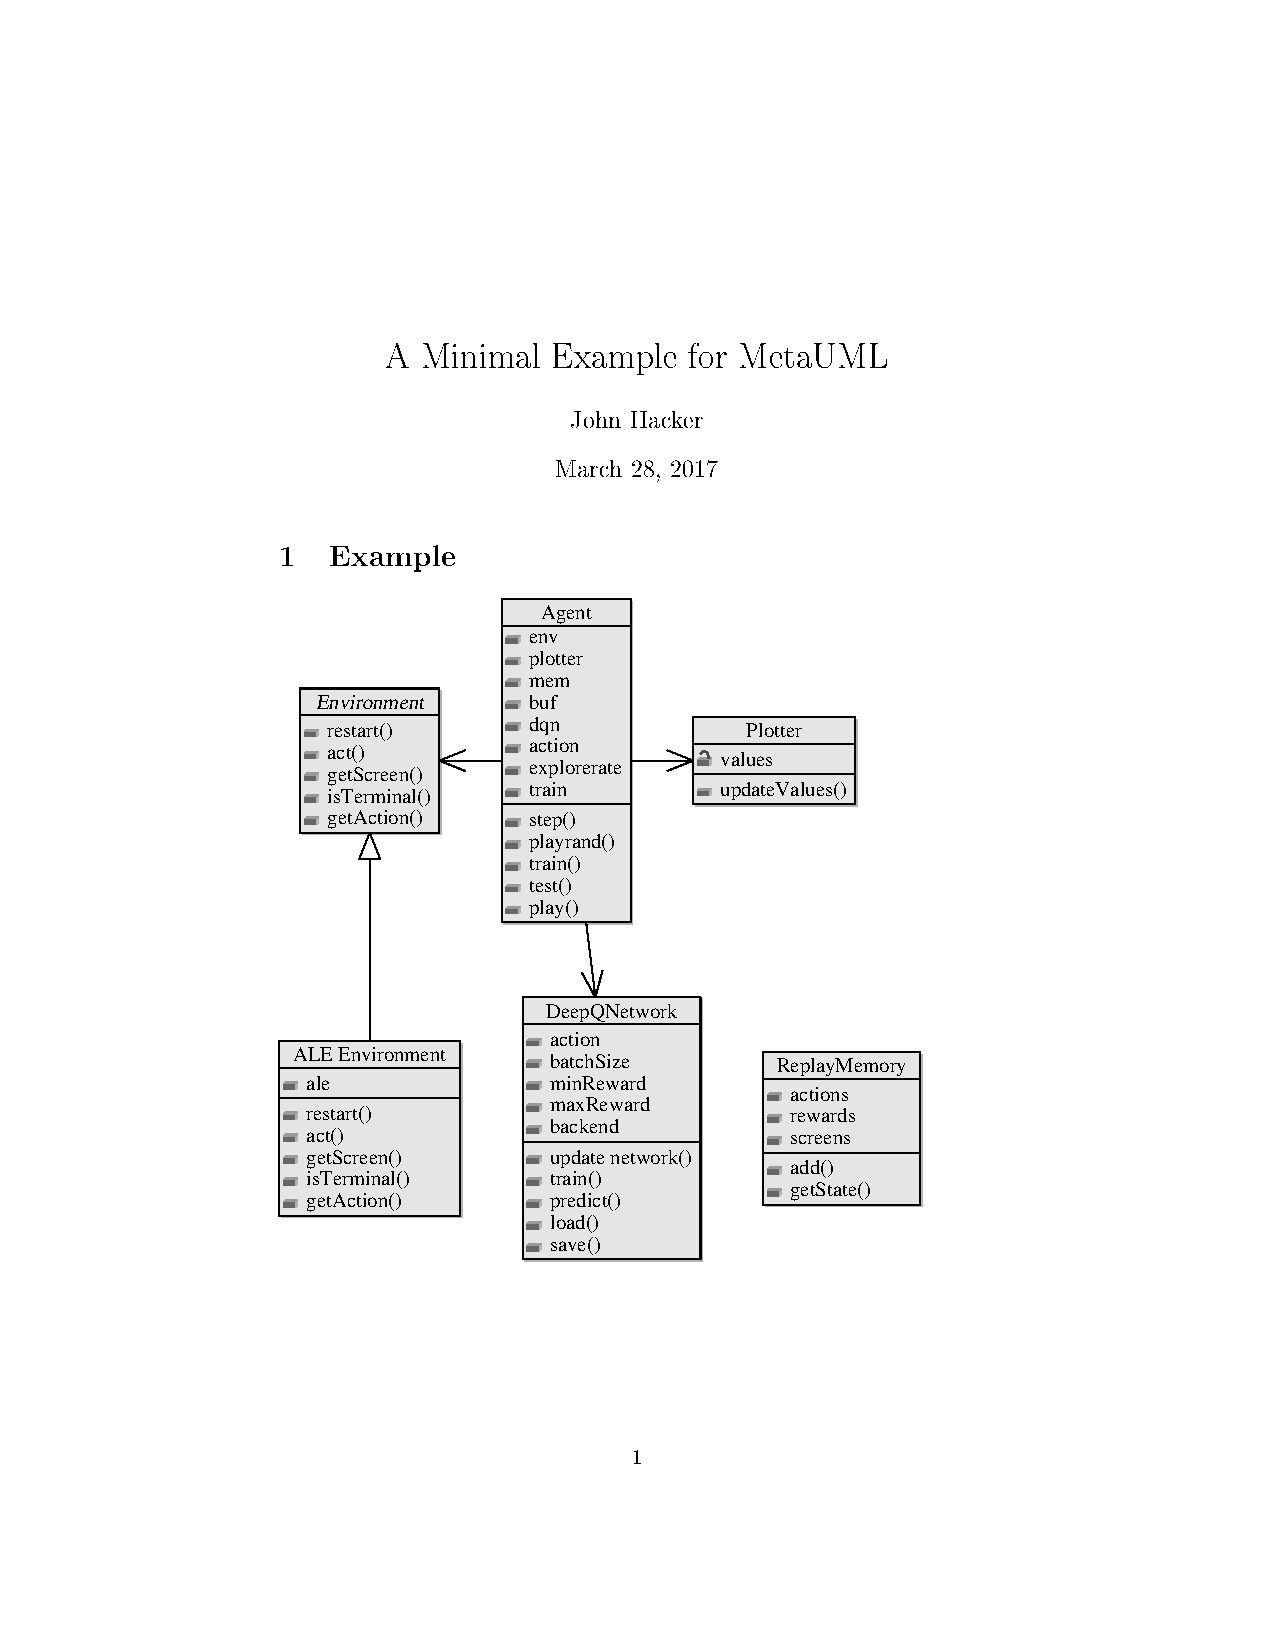
\includegraphics[width=15cm]{../uml/uml.1}\\
						\caption{UML Class Diagram.}
					\end{centering}
				\end{figure}

		\section{Code Overview}
			The code for the project is open on github. https://github.com/devilsangel/deepQLearning

			\subsection{Environment}
				The environment is an interface that is used to control the environment of the game. It gives the actions that can be peformed at any given time, gets the current state of the system, act a particular action on the system and return the reward if there is one. It also alerts the agent when a terminal state is reached.

				The ALEEnvironment is the class that implements the environment interface. The structure was made so that different environments could be used interchangably with minimal change to the code. Other environments like gym environment can be used to implement the interface as well.

			\subsection{Agent}
				Agent class is the crux of the system. Which has variables of all other class types. In train mode, the system trains based on the qvalues provided by the deepQNetwork occasionally correcting it when rewards approach. After every step of the game, a callback to statisctics on step function is called. During training the loss of a life or the end of the game is treated as terminal states. Exploration rate controls whether exploration or exploitation is chosen. 

				In test mode, a given no of games are played, here the statebuffer is used to disallow contamination of trained data. Here only the end of the game is taken as a terminal state.

				In random mode, random actions are given to the system and the output observed.

			\subsection{Plotter}
				The plotter class uses python libraries to plot the data saved about each epoch as a graph. Visualising the important data metrics like average score and qvalue of each epoch, which can be used to evaluate the performance of the training.

				It also serves the function of plotting the maximum qvalue of the current screen live during play.
			
			\subsection{Statistics}
				The statistics class embeds itself as a callback in the agent class. The agent calls the on step method after every step of the game. If the game reaches a terminal state, the values like average score, no of games etc are updated in the statistics class.

				When the epoch ends, the write method is called which appends the calculated data to the csv file.

			\subsection{DeepQNetwork}
				An abstraction layer over Neon, a deep learning library from Nervana Systems. It Models the Network, finds the Q values associated with a state of the system, and does updation of weights based on reward and a random minibatch. The reward is used to refine the discounted future reward of the minibatch.

			\subsection{Replay Memory}
				For training the states, actions, screens and rewards need to be saved. These can be added to the replay memory using the add method. When a reward is obtained, a minibuffer is selected with the current state at the index position. This minibuffer is used for training the system.

			\subsection{State Buffer}
				During testing and play, the replay memory is not necessary, so a stripped down version of it, storing only the states of the system is used. This has the added advantage of ensuring that the data from testing does not pollute the training data.

	\chapter{Results and Discussions}
		The results of the training sessions were saved in a csv file in increments of 1 epoch or 250000 steps. Important parameters of the epoch like steps, number of games, average reward, mean cost, average q value etc are saved for three phases, training, test and random.


		\section{Description of observed strategies}
			\subsubsection{Breakout}
				Before training the system plays randomly, \emph{ie} chooses an action at random. 

				After one epoch the system adopts a simple strategy, to move to the left of the screen and stay there, an approach that assures a minimum score of two before defeat.

				After ten epochs the system plays like a human player, moving the paddle in response to the ball and dropping it occasionally.

				At fifty epochs, the play is significantly better occasionally resorting to the top strategy of tunnelling to the top of the screen from the edge.

			\subsubsection{Space Invaders}
				Space Invaders was trained for 8 epochs to prove that the algorithm can be used to train and play multiple games without any alterations proving the general purposse nature of it. At 8 epochs the game is played as a human would hitting the targets accurately enough and a consistent score in the range of 400 to 800 is obtained by the system.

		\section{Result Visualization}

			The results stored in csv files were plotted as a graph for visualization using matplotlib python module. Training was done for 50 epochs (65 hours). The games adopt visibly better strategies on later epochs. Space Invaders was trained with the same algorithm without any change, thus proving the general purpose nature of the algorithm.
			
			\newpage
			\subsubsection{Breakout}

			\begin{figure}[H]
				\begin{centering}
					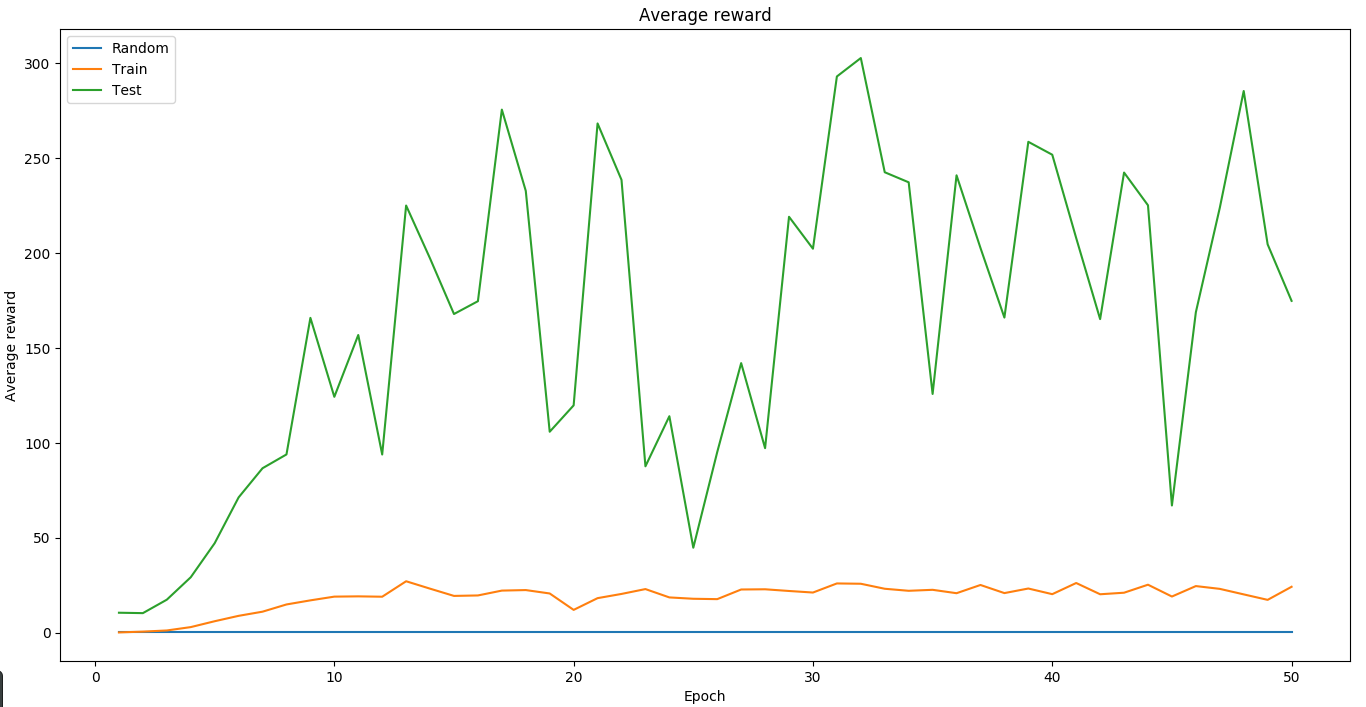
\includegraphics[width=15cm]{images/breakout_1_average_reward.png}
					\caption{Average Reward per epoch - Breakout.}
				\end{centering}
			\end{figure}			
			
			\begin{figure}[H]
				\begin{centering}
					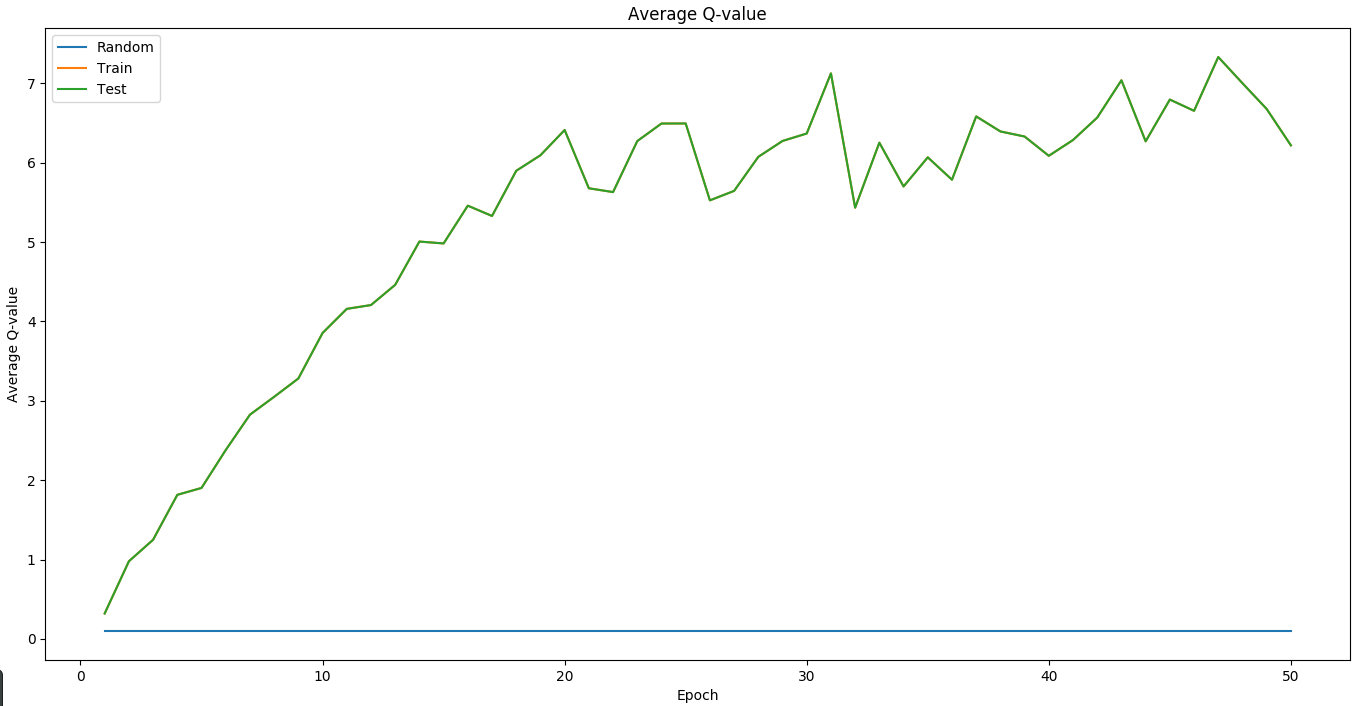
\includegraphics[width=15cm]{images/breakout_2_meanq.png}
					\caption{Mean Q Value per epoch - Breakout.}
				\end{centering}
			\end{figure}			
			
			\begin{figure}[H]
				\begin{centering}
					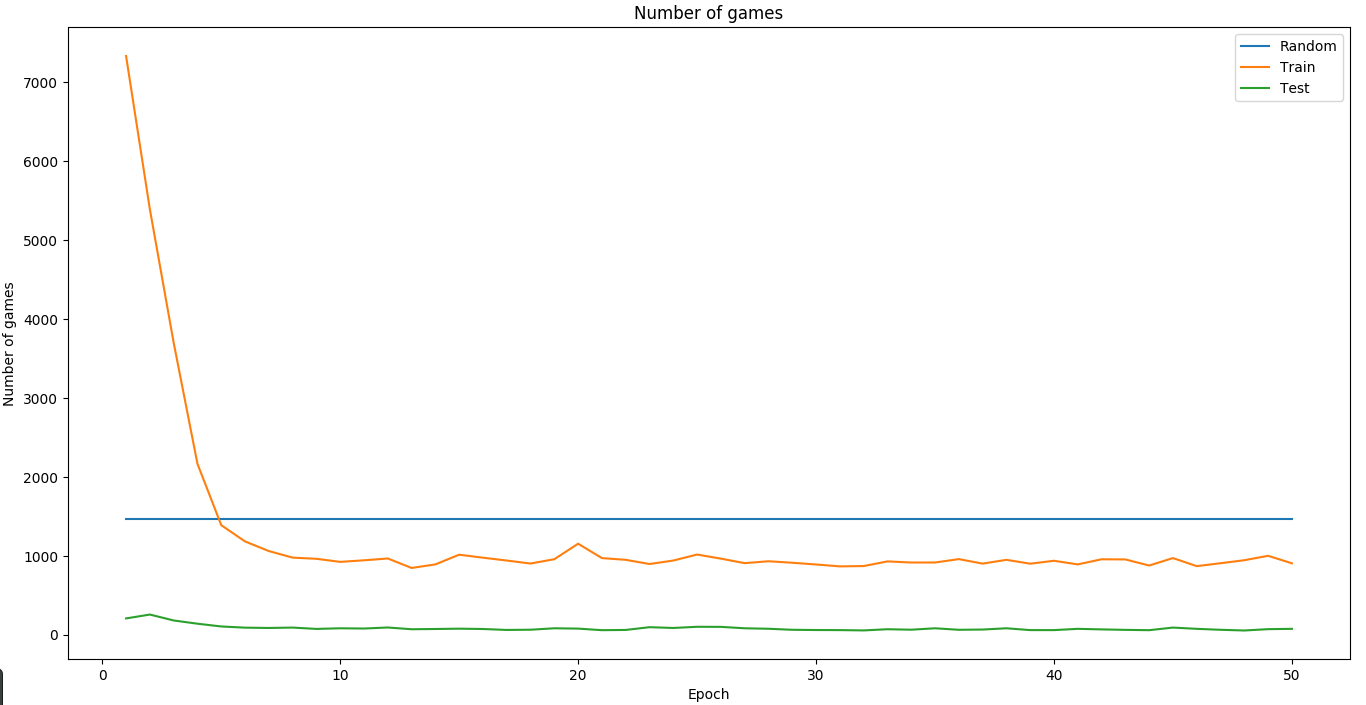
\includegraphics[width=15cm]{images/breakout_3_nrgames.png}
					\caption{No of games per epoch - Breakout.}
				\end{centering}
			\end{figure}			
			
			\begin{figure}[H]
				\begin{centering}
					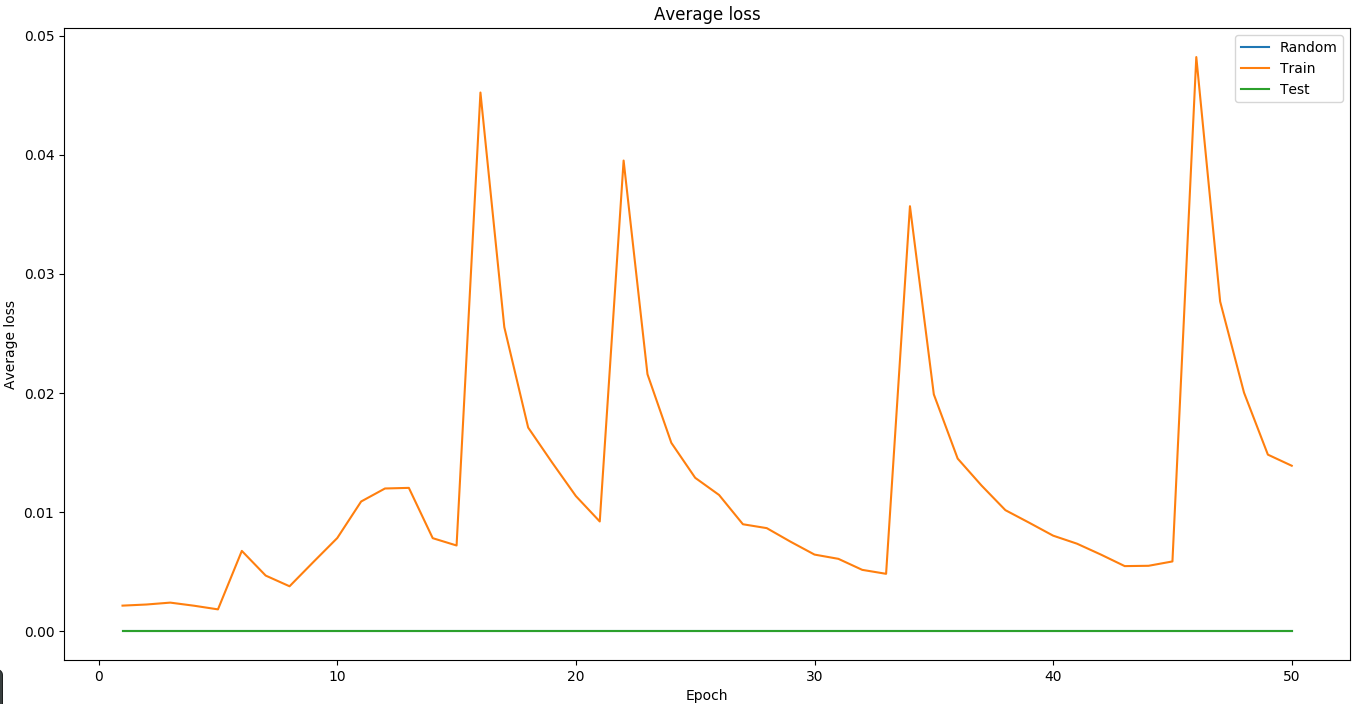
\includegraphics[width=15cm]{images/breakout_4_averageloss.png}
					\caption{Average loss per epoch - Breakout.}
				\end{centering}
			\end{figure}			
			
			\newpage
			\subsubsection{Space Invaders}

			\begin{figure}[H]
				\begin{centering}
					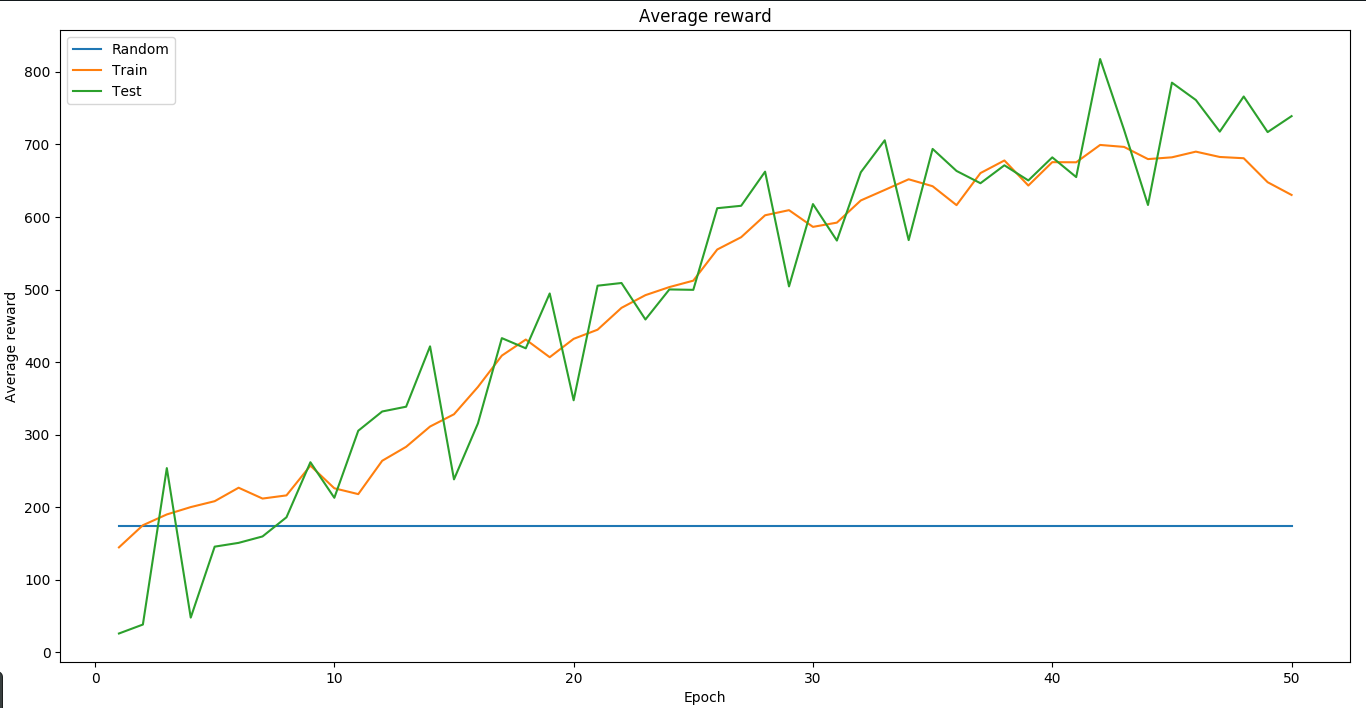
\includegraphics[width=15cm]{images/space_1_average_reward.png}
					\caption{Average Reward per epoch - Space Invaders.}
				\end{centering}
			\end{figure}			
			
			\begin{figure}[H]
				\begin{centering}
					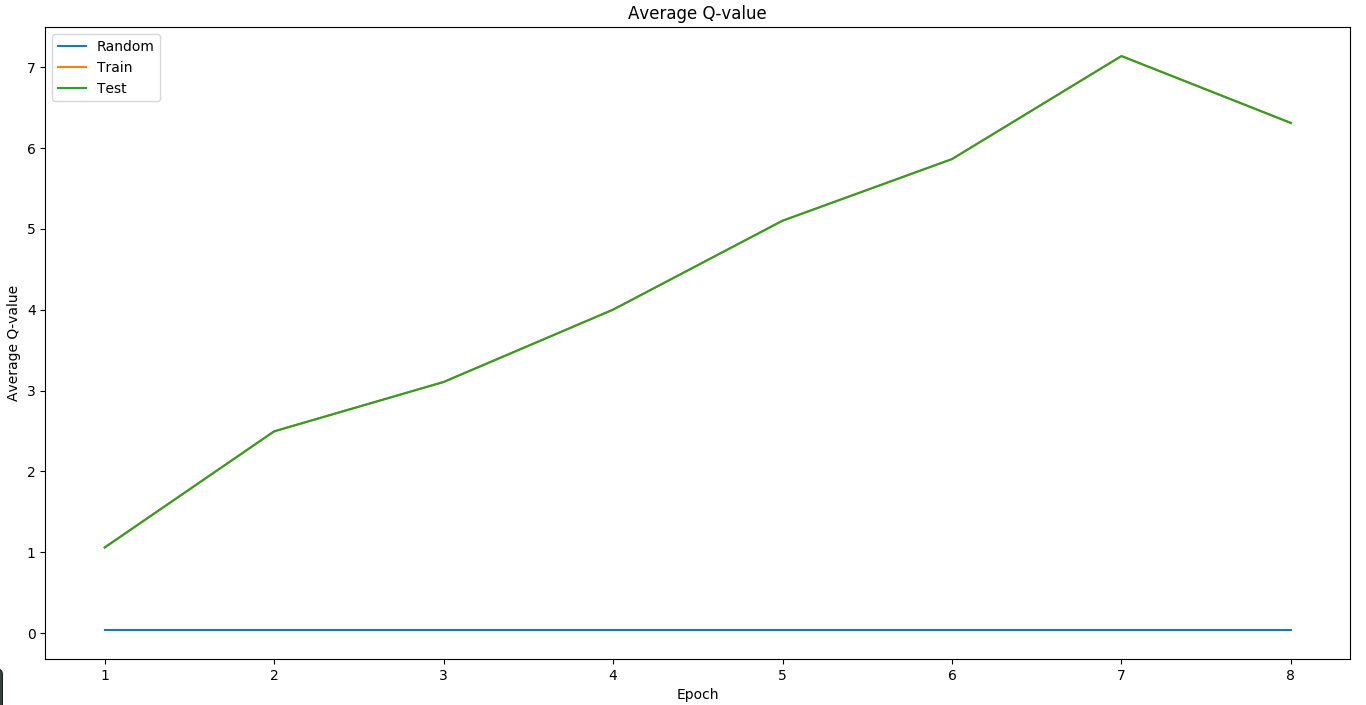
\includegraphics[width=15cm]{images/space_2_meanq.png}
					\caption{Mean Q Value per epoch - Space Invaders.}
				\end{centering}
			\end{figure}			
			
			\begin{figure}[H]
				\begin{centering}
					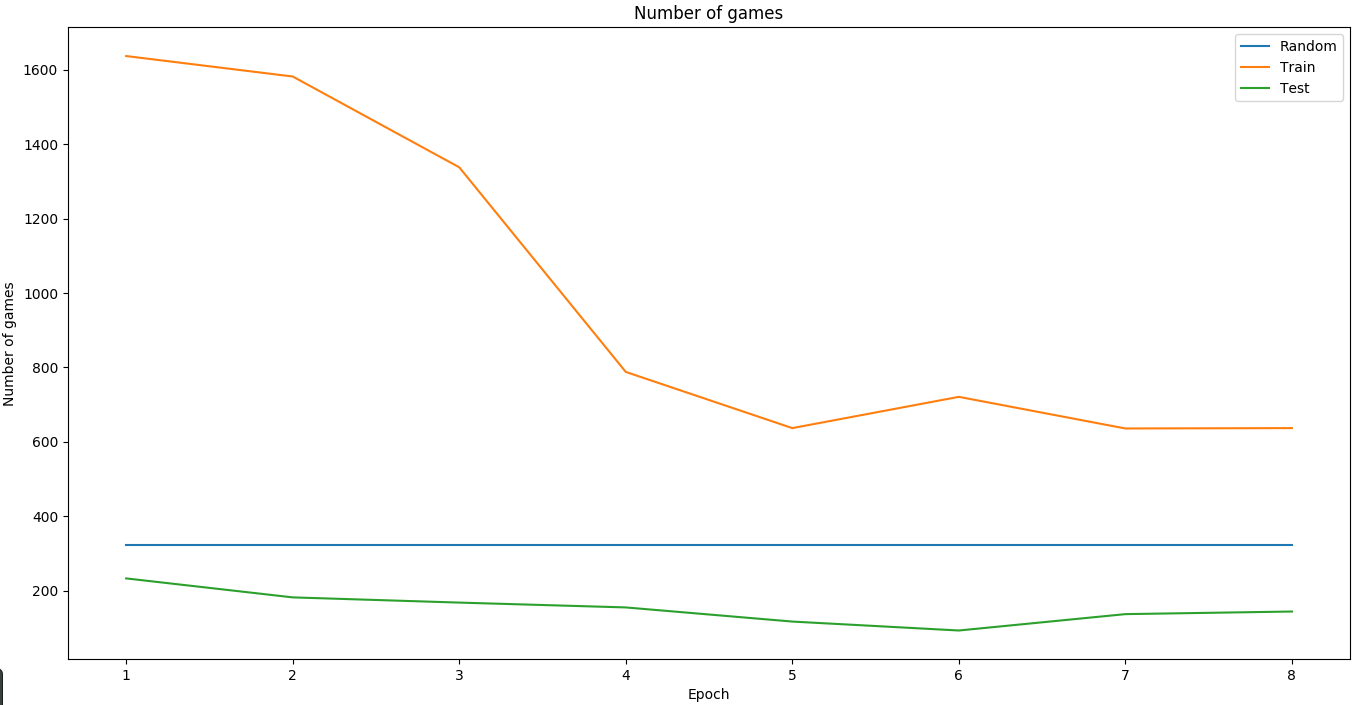
\includegraphics[width=15cm]{images/space_3_nrgames.png}
					\caption{No of games per epoch - Space Invaders.}
				\end{centering}
			\end{figure}			
			
			\begin{figure}[H]
				\begin{centering}
					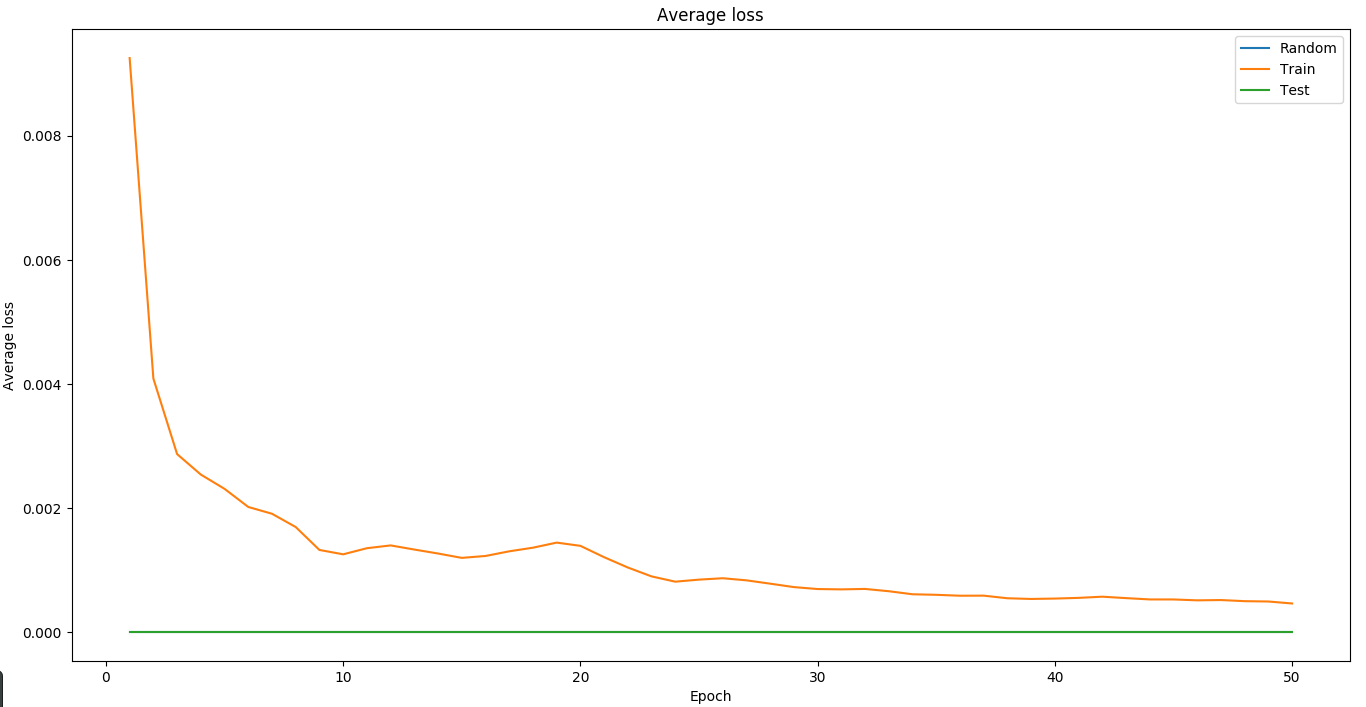
\includegraphics[width=15cm]{images/space_4_averageloss.png}
					\caption{Average loss per epoch - Space Invaders.}
				\end{centering}
			\end{figure}			
			



	\chapter{Further Work}
		\section{Gamification of Problem}
			Solving real world problems can be achieved using Deep Reinforcement Learning. The following points are to be considered to convert a real world problem into a deep learning optimisation problem:
			\begin{itemize}
				\setlength\itemsep{0em}
				\item The problem is to be modelled as a game.
				\item The game should include an environment which has a finite set of actions.
				\item High dimensional input to the environment should be available as input and savable as a state.
				\item State of the system should change according to the actions performed on it.
				\item The environment should occasionally give off rewards in response to its current state or action performed.
			\end{itemize}

			If all of the criterions are met and a gamified version of the real world problem is made, then it can be quite easily given to a deep reinforcement learning system for optimisation and then later used in real life after training.

		\section{Traffic Light Control}
				A sample real world problem that could be solved using reinforced learning.
			\subsection{Problem}
				There is an intersection of two roads, and four traffic lights control the traffic in it, each controlling one road. The control of the traffic light should be given to an \ac{ai} for optimum traffic flow through the intersection. To design a system that can be used to train this \ac{ai}. 

			\subsection{Minimal Input}
				Traffic camera images at four different directions are taken as input to the system, mulitple images are taken to incorporate movement of the vehicles. Even though the system could work with the raw images, it would be impossible to train the system in the real world. So a simulation is required to train it. But in a simulation output images cannot be generated as complex as real video stream. 

				The solution is to simplify the input to the system, and to simulate the output in this simplified version. The approach taken is to convert the vehicles into white rectangles in a black canvas, and the intersection as a line. Thus white rectangles passing over the line will be taken for rewards and any intersection of rectangles will be interpreted as a crash. The rectangles are easier to simulate given the actions to be performed.

				To make the simulation closer to reality, delay between the signal turning green and the first car moving can be given. Contraction and elongation of traffic at stop and start can also be simulated.

				\begin{figure}[H]
					\begin{centering}
						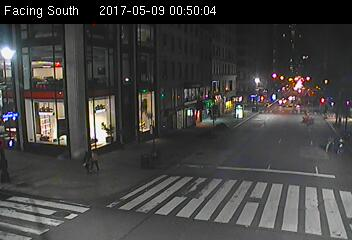
\includegraphics[width=10cm]{images/traffic1.png}
						\caption{Empty Intersection.}
					\end{centering}
				\end{figure}

				
				\begin{figure}[H]
					\begin{centering}
						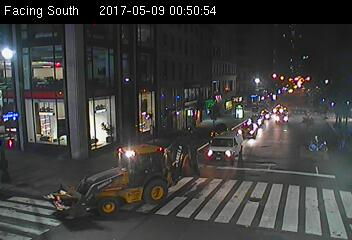
\includegraphics[width=10cm]{images/traffic2.png}
						\caption{Intersection with Vehicles.}
					\end{centering}
				\end{figure}

				
				\begin{figure}[H]
					\begin{centering}
						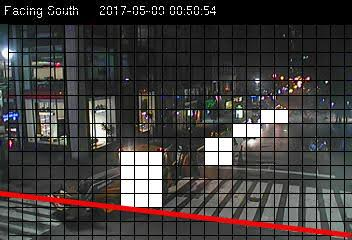
\includegraphics[width=10cm]{images/traffic3.png}
						\caption{Generation of Simplified Input.}
					\end{centering}
				\end{figure}

				
				\begin{figure}[H]
					\begin{centering}
						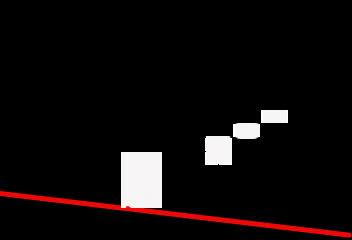
\includegraphics[width=10cm]{images/traffic4.png}
						\caption{Simplified Input.}
					\end{centering}
				\end{figure}



			\subsection{Action set}
				At any instant, any of the traffic lights can be any of the following:
				\begin{itemize}
					\setlength\itemsep{0em}
					\item Red
					\item Orange
					\item Green in the Right, Left or Straight direction or any combination of it.
				\end{itemize}

				Orange can be eliminated by making it mandatory for transitions between Green and Red. Green has seven states (not to be confused with state of the system found from the input) it can be in for all the combinations. Since only Green or Red can be active at a given time, the total no of states for a single traffic light is 8.

				The intersection consists of 4 traffic lights, operating independantly (No constraints to its operation) making the total no of actions the system can take to $8^4$ \emph{ie} 4096 actions.

				Thus at every state of the system, it can decide between 4096 actions to take.
			\subsection{Reward}
				The no of vehicles that pass through the intersection in a time interval or the throughput of the intersection can be taken as a rudimentary reward function.

				To avoid any traffic signals that might incur collisions, any collisions detected are penalised with a negative reward. This still presents the problem of starvation \emph{ie.} a low amount of vehicles could wait for green indefinitely. It can be solved by aging the throughput negatively, which makes the throughput reward smaller and finally negative the longer it waits.
			\subsection{Scalability}
				The system proposed could be implemented on a larger scale, like a town or city. But in the current form of neural networks, adding a single traffic light to an existing system makes retraining the entire system a requirement. As the number of intersections increase, the number of actions rise exponentially. Thus making their efficient implementation a problem.

				The bottleneck is the non scalability of the current architecture, which could be tentatively solved if parallel neural networks are introduced. Parallel neural networks are still in its infancy and outside the scope of this project.
	\chapter{Conclusion}
		It is clear from the results that the presented model can used in applications with high dimensional sensory input. They also show that the algorithm will eventually converge to an optimal policy. Real world problems can be modelled as an environment with reward and actions, and plugged into the algorithm.

		Lack of processing power was observed as a pertinent limitation. The deepLearning library, Neon is optimized for Nvidia Maxwell Graphic Processing Units and its performance is very low on CPUs and pre-maxwell GPUs. We experimented training on GeForce GT 735M, Jetson TX1 board, and an i3 desktop CPU, the best among these was the GT 735M which took 77 mins per epoch.


	\newpage
	\nocite{*}
	\bibliography{helpers/bibliography}
	\bibliographystyle{ieeetr}

\end{document}